\documentclass{beamer}
\usepackage[autokw=all]{svn-multi}
\setbeamertemplate{navigation symbols}{}
%\usetheme{Goettingen}
\usetheme{Malmoe}
\usefonttheme{default}
%\setbeamersize{text margin left=5pt,text margin right=5pt}

\usepackage{hyperref}
\usepackage{subfigure}
\usepackage{amsmath}
\usepackage{amssymb}
\usepackage{multimedia}
\usepackage{shadow}
%\usepackage{movie15}

\usepackage{tcolorbox}

% Create a ``Wider'' command to reduce margins.  Put
% ``\Wider{\lipsum[2]}'' in a frame...
\newcommand\Wider[2][3em]{%
\makebox[\linewidth][c]{%
  \begin{minipage}{\dimexpr\textwidth+#1\relax}
  \raggedright#2
  \end{minipage}%
  }%
}


%\usepackage[english]{babel}
%\usepackage{pgf,pgfarrows,pgfnodes,pgfautomata,pgfheaps}
% \usepackage[latin1]{inputenc}

\usepackage{graphicx}
\defbeamertemplate*{footline}{default theme}
{
  \leavevmode%
  \hbox{%
  \begin{beamercolorbox}[wd=.5\paperwidth,ht=2.25ex,dp=1ex,center]{author in head/foot}%
    %\usebeamerfont{author in head/foot}\insertshortauthor~~(\insertshortinstitute)
    \usebeamerfont{author in head/foot}\insertshortauthor
  \end{beamercolorbox}%
  \begin{beamercolorbox}[wd=.4\paperwidth,ht=2.25ex,dp=1ex,center]{title in head/foot}%
    \usebeamerfont{title in head/foot}\insertshorttitle
  \end{beamercolorbox}%
  \begin{beamercolorbox}[wd=.1\paperwidth,ht=2.25ex,dp=1ex,right]{date in head/foot}%
%    \usebeamerfont{page number}\insertframenumber{} / \inserttotalframenumber\hspace*{2ex} 
    \usebeamerfont{page number}\insertpagenumber{} / \insertpresentationendpage{} \hspace*{2ex} 
  \end{beamercolorbox}}%
  \vskip0pt%
}

\title{Software for Mind Control}

\author{Ben Pearre}
%\institute[]{
%  Computer Science\\
%  University of Colorado at Boulder, USA}
\date{\today\\{\small (Rev. \svnrev)}}
%\date{\today}

\begin{document}

\begin{frame}
  \titlepage
\end{frame}

\begin{frame}
  \frametitle{Outline}
  \tableofcontents
\end{frame}


%\begin{frame}
%  \outline
%\end{frame}


\section{Introduction}
\subsection{Goals}

\begin{frame}
  \frametitle{Goals}
  \begin{itemize}
  \item Goal-directed modification of behaviour
    \begin{itemize}
    \item Optimise stimulation parameters
      \begin{itemize}
      \item Learn to produce desired output
      \item Minimise voltage
      \end{itemize}
    \end{itemize}
  \item Demonstrate chronically implanted electrodes
  \item Safely stimulate despite small surface area
  \end{itemize}
\end{frame}


\subsection{Tools --- hardware}

\begin{frame}
  \frametitle{Electrodes}
  \begin{columns}
    \column{6cm}
    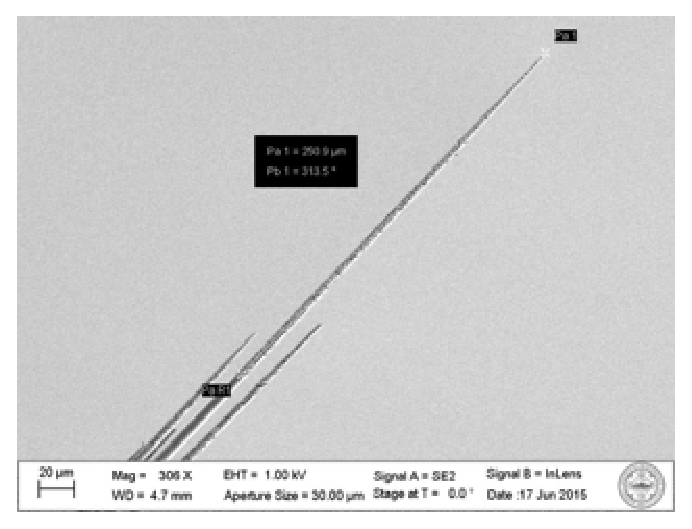
\includegraphics[width=\textwidth]{electrodes_up_close}
    \column{4cm}
    Chronic high-count high-impedance\dots
    \begin{itemize}
    \item Carbon fibres
    \item Silicon carbide
    \item Optical\dots?
    \end{itemize}
  \end{columns}
\end{frame}

\begin{frame}[plain]
  \begin{center}
    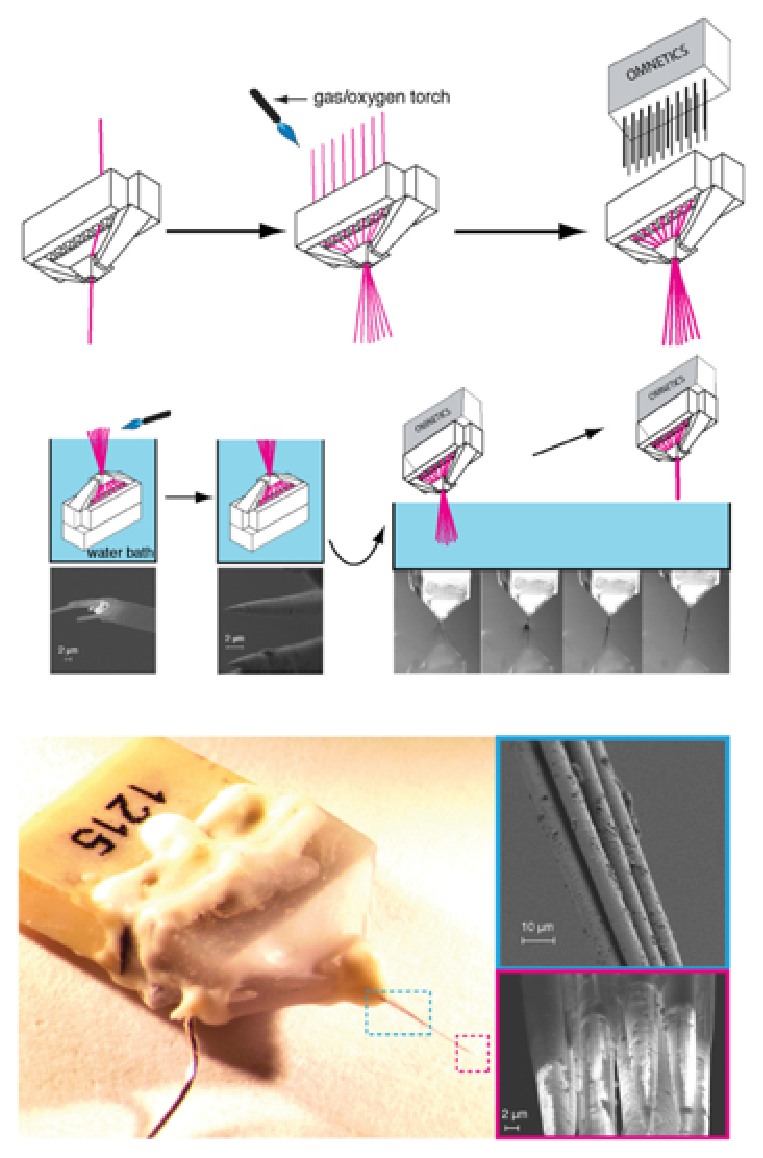
\includegraphics[height=\textheight]{julia_electrodes}
  \end{center}
\end{frame}

\begin{frame}[plain]
  \includegraphics<+>[width=\textwidth]{CFHistSplayFronSanneImg1}
  \includegraphics<+>[width=\textwidth]{CFHistSplayFronSanneImg2}
\end{frame}


\begin{frame}
  \frametitle{Plexon stimulator}
  \begin{itemize}
    \item 16 channels
    \item Current-controlled
    \item Externally triggered
    \item Arbitrary pulse waveforms
    \item Resolution: 30 nA $\times 1 \mu$s
    \item Matlab API
    \item Reprogramming time $\approx$ 0.1s/channel (?)
    \item Voltage monitoring is expensive!
  \end{itemize}
\end{frame}

\section{Experiment}

\begin{frame}
  \frametitle{Antedromic HVC$\leftarrow$X response}
  \includegraphics<+>[width=\textwidth]{hvc_areaX}
  \includegraphics<+>[width=\textwidth]{plexme}
\end{frame}

\section{Results}

\subsection{Chronic recording}

\begin{frame}
  \frametitle{Recording --- IrO$\textsubscript{2}$ in X}
  197 days post-surgery
  \includegraphics[width=\textwidth]{spiketrain-lw95rhp-2015-11-19}
  
  \includegraphics[width=\textwidth]{spiketrain-lw95rhp-2015-11-23}
\end{frame}

\begin{frame}
  \frametitle{Recording --- bare carbon in X}
  234 days post-surgery
  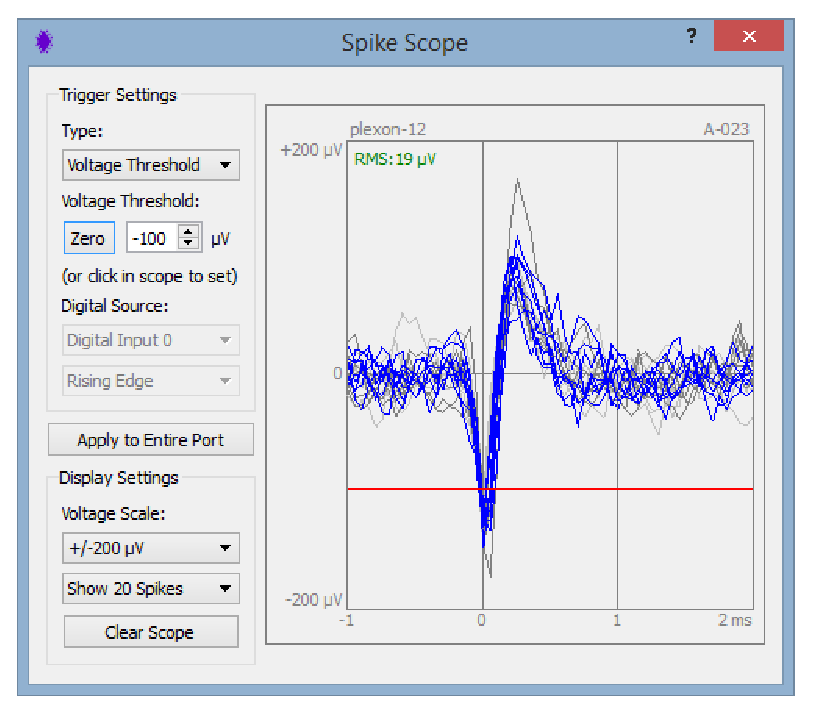
\includegraphics[height=\textheight]{lw85ry_x}
\end{frame}


\subsection{Current Steering}


\begin{frame}
  \frametitle{Previous work}
  \begin{columns}
    \column{5cm}
    \column{5cm}
    \begin{itemize}
    \item Fast
    \item Wrong
    \end{itemize}
  \end{columns}
\end{frame}


\begin{frame}
  \frametitle{Voltage minimisation}
  \includegraphics<+>[width=\textwidth]{current_steering_voltages}
  \includegraphics<+>[width=\textwidth]{current_steering_voltages_valid}
\end{frame}

\begin{frame}
  \frametitle{Response shaping in HVC}
  \includegraphics[width=\textwidth]{current_steering_hvc_responses}
  
  \includegraphics[width=\textwidth]{current_steering_hvc_responses_std}
\end{frame}





%%% Future! %%%
\section{The Future!}
\subsection{Ideas}

\begin{frame}
  \frametitle{Stimulation optimisation}
  \begin{columns}
    \column{35mm}
    Criteria?
    \begin{itemize}
      \item Minimise voltage
      \item See response (binary?)
      \item Correlation maximisation
      \item Response separation
      \item Directed change to song
        \begin{itemize}
          \item Acute
          \item Chronic
        \end{itemize}
    \end{itemize}
    \column{35mm}
    Policy outputs?
    \begin{itemize}
      \item Pulse train timing
      \item Channel timing
      \item Arbitrary pulse shape
    \end{itemize}
    \column{35mm}
    Policy inputs?
    \begin{itemize}
      \item Vocalisation
      \item Other motor output?
      \item Neural activity
    \end{itemize}
  \end{columns}
\end{frame}


\subsection{Electrodes}
\begin{frame}
  \includegraphics<+>[width=\textwidth]{stuart}
\end{frame}


\end{document}
